\newpage
\section{Auswertung}
\label{sec:Auswertung}
\subsection{Statische Methode}
\label{sec:Statische}
Aus den gemessenen Werten der statischen Methode bestimmt sich die Winkelrichtgröße nach Formel \eqref{eqn:D}, zu finden in Tabelle \ref{tab:D}.
\begin{align}
\intertext{Der Abstand von der Drehachse beträgt:}
 r=0,1375\,\si{\meter}.
\end{align}
Desweiteren wurden ein Fehler von $5°$für die Winkelmessung angenommen, da der Winkel nur durch fehlerbehaftetes Ablesen gemessen wurde.
Der in rad ungefähr $0,09$ rad beträgt.
Die errchneten Werte werden gemittelt und es ergibt sich eine Winkelrichtgröße von:
\begin{align}
  D=(0,044\pm0,010)\,\si{\newton\meter}
\end{align}
\begin{table}
 \centering
 \caption{Messwerte für die Federkonstante $D$ }
 \label{tab:D}
 \begin{tabular}{c c c}
\toprule
Auslenkwinkel $ \varphi\:/\:\text{rad} $      & $F\:/\:\si{\kilo\gram\meter\per\second\squared}$
& $D\:/\:\si{\kilo\gram\meter\squared\per\second\squared}$\\
\midrule
0,52\pm 0,09  &   0,09\pm 0,03   &   0,024\pm 0,008\\
0,87\pm 0,09  &   0,37\pm 0,03   &   0,058\pm 0,005\\
1,05\pm 0,09  &   0,38\pm 0,03   &   0,050\pm 0,004\\
1,22\pm 0,09  &   0,50\pm 0,03   &   0,056\pm 0,003\\
1,57\pm 0,09  &   0,52\pm 0,03   &   0,046\pm 0,003\\
2,09\pm 0,09  &   0,70\pm 0,03   &   0,046\pm 0,002\\
2,62\pm 0,09  &   0,75\pm 0,03   &   0,039\pm 0,002\\
3,14\pm 0,09  &   0,85\pm 0,03   &   0,037\pm 0,001\\
3,67\pm 0,09  &   0,95\pm 0,03   &   0,036\pm 0,001\\
4,19\pm 0,09  &   1,45\pm 0,03   &   0,048\pm 0,001\\
\bottomrule
\end{tabular}
\end{table}


\subsection{Dynamische Methode}
\label{sec:Dynamische}
Die Messwerte für die Dynamische Methode sind in dem Abb.\ref{abb:b} in der Form $T^2$ gegen $a^2$ aufgetragen.
Es besteht ein linearer Zusammenhang zwischen $T^2$ und $a^2$
wie in der Formel \eqref{eqn:cool}.
\begin{align}
I  &= 2(I_{\mathrm{z}}+m\cdot a^2) \\
D\cdot \frac{T^2}{4\pi^2}-I_{\mathrm{D}} &= 2(I_{\mathrm{z}}+m\cdot a^2)
\intertext{durch einstetzen der Formel \eqref{eqn:I} und umformen nach $a^2$ ergibt sich} %
a^2 &= D_{\mathrm{dyn}}\cdot \frac{T^2}{8\pi^2m}-\frac{I_{\mathrm{D}}}{2m}-\frac{I_{\mathrm{z}}}{m}\label{eqn:cool}
\intertext{Durch die Lineareregression lässt sich mit dem  Y-Achsenabschnitt  $a$ berechnen und somit durch Umformen  $I_{\mathrm{D}}$ bestimmen:}
a&=-\frac{I_{\mathrm{z}}}{m}-\frac{I_{\mathrm{D}}}{2m}\\
I_D&=-2ma-2I_z
\intertext{Durch einsetzten des Trägheitsmoments des Zylinders \eqref{eqn:zl} ergibt sich}
I_{\mathrm{D}}&=-2ma-2m\left(\frac{\left(\frac{d_{\mathrm{{z}}}}{2}\right)^2}{4}+\frac{h_{\mathrm{z}}^2}{12}\right)
\intertext{Durch Einsetzen der gemittelten gemessenen Größen}
 m&=(0,2225\pm0,000005)\, \si{\kilo\gram}\\
 d_{z1}&=(0,03494\pm0,00003)\,\si{meter}\\
H_z&=0,0300\pm0,00006\,\si{meter}
\intertext{ergibt sich für das Trägheitsmoment der Drillachse}
I_D&=(0,0027454\pm0,0000002)\,\si{\kilo\gram\meter\tothe{2}}
\intertext{Ebenfalls lässt sich mit Hilfe der aus der Linearenregression berechneten Steigung $b$ die dynamische Winkelrichtgröße $ D_\mathrm{dyn}$ bestimmen:  }
b=\frac{D_\mathrm{dyn}}{8\pi^2m}.\\
D_\mathrm{dyn}=8a\pi^2m.\\
\intertext{Durch einsetzen der Werte ergibt sich}
D_\mathrm{dyn}=(0,0295\pm0,0004)\, \si{\kilo\gram}.\\
Da sich die dynamische Winkelrichtgröße von der statisch gemessenen Winkelrichtgröße unterscheidet, wird die dynamische Winkelrichtgröße im
folgendem Teil als Winkelrichtgröße verwendet, da die folgenden Trägheitsmoment ebenfalls mit der Dynamischen Medthode bestimmt werden.
\end{align}
\begin{figure}
   \centering
   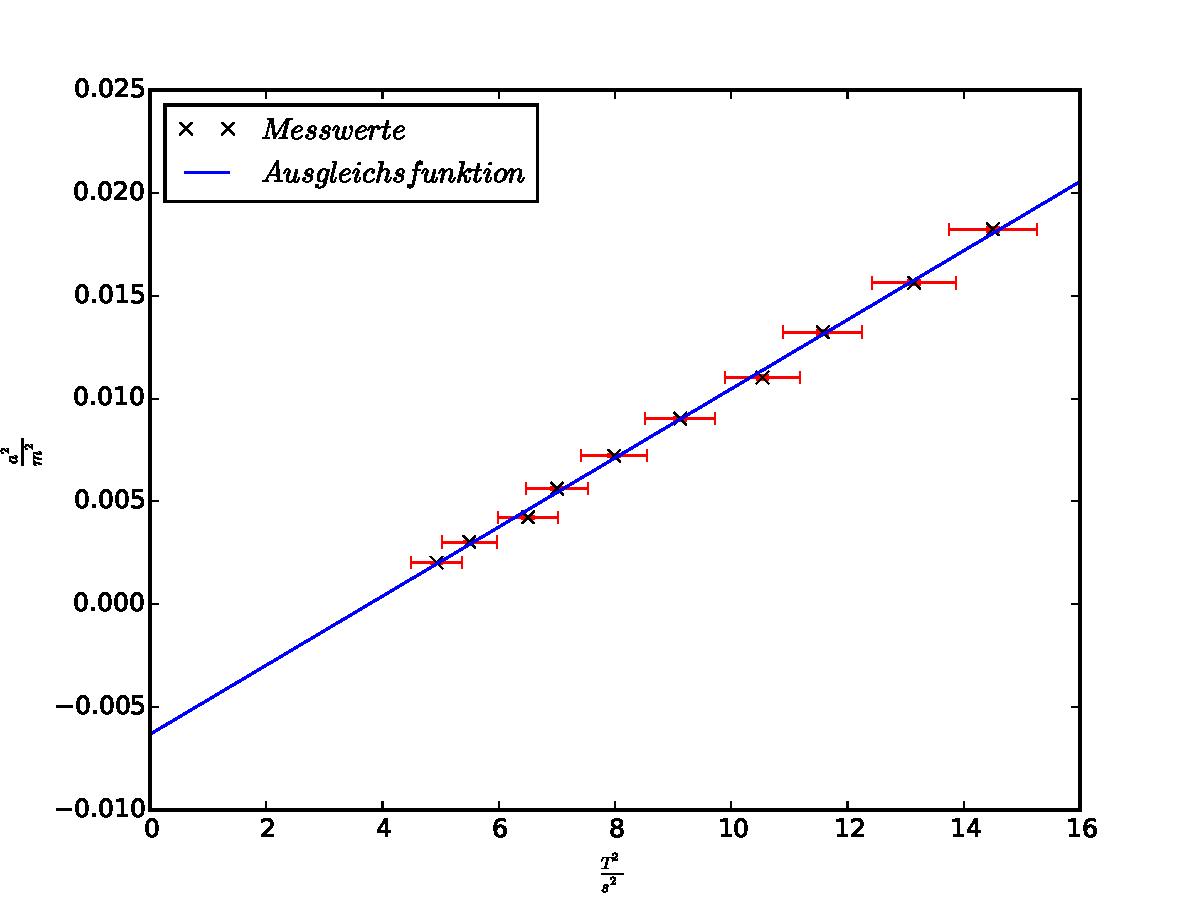
\includegraphics[width=0.7\textwidth]{b.pdf}
  \caption{Das Abstandsquadrat $a^2$ in Abhängigkeit von dem Periodendauerquadrat $T^2$ }
  \label{abb:b}
\end{figure}
\newpage
\subsection{Trägheitsmoment von geometrischen Figuren}
\subsubsection{Zylinder}
Nun werden die Werte für das Trägheitsmoment eines Zylinder,
mit der Masse
\begin{align*}
m=(1,9739\pm0,00005)\,\si{\meter}
\end{align*}
einmal mit der Formel  \eqref{eqn:I}
aus den Messwerten berechnet.
Dafür werden die gemessenen Zeiten gemittelt,
\begin{align*}
T\overline= (1,455\pm0,016)\,\si{\second}\\
\intertext{und es ergibt sich ein}
I_{\mathrm{gemessen}}=(-0,0004\pm0,0005)\,\si{\kilo\gram\meter\squared}.
\end{align*}
Aus der Theoretischenformel \eqref{eqn:zs} für
einen Zylinder der parallel zur Drehachse verläuft mit dem Durchmesser
\begin{align*}
  d_{z2}=(0.08019\pm0.00011)\,\si{\meter},
\intertext{ergibt sich eine theoretisches Trägheitsmoment}
I_\mathrm{theorie}= 0.0003011\pm0.0000006\,\si{\kilo\gram\meter\squared}.
\intertext{Somit beträgt die Abweichung von Theoriewerte die mit der Formel \eqref{eqn:abweich} berechnet wird}
a=(425\pm13)\,\si{\percent}.
\end{align*}
\subsubsection{Kugel}
Dies mal werden die Werte für das Trägheitsmoment eine Kugel,
die die Masse $(m=0,8125\pm0,00005)\si{\meter} $ besitzt, wieder mit der Formel  \eqref{eqn:I}
aus den Messwerten und aus der Theoretischenformel \eqref{eqn:Kugel} für eine
Kugel mit dem Durchmesser
\begin{align}
  d_{k}=(0.1365\pm0.0019)\si{\meter}
\end{align}
berechnet. Diese sind in Tabelle \ref{tab:Kugel} dargestellt.
\begin{table}
 \centering
 \caption{Messwerte und Theoriewerte für die Kugel}
 \label{tab::Kugel}
 \begin{tabular}{c c c}
\toprule
$\frac{T}{\si{\second}}$      & $\frac{I_{gemessen}{\si{\kilo\gramm\meter\squared}}}$
& $\frac{I_{theorie}{\si{\kilo\gramm\meter\squared}}}$
\midrule
1.486\pm 0.1  &  -0.0001 \pm0.0006 &  0.001514757\pm 0.00004\\
1.498\pm 0.1  &  -0.0001 \pm0.0006 &  0.001514757\pm 0.00004\\
1.482\pm 0.1  &  -0.0001 \pm0.0006 &  0.001514757\pm 0.00004\\
1.476\pm 0.1  &  -0.0002 \pm0.0006 &  0.001514757\pm 0.00004\\
1.486\pm 0.1  &  -0.0001 \pm0.0006 &  0.001514757\pm 0.00004\\
\bottomrule
\end{tabular}
\end{tablel}

\newpage
\subsection{Trägheitsmoment einer Puppe}
Der Körper der Puppe wird mit verschiedenen Zylindern genähert, wie in Abbildung \ref{fig:puppe} zu sehen.
\begin{figure}
 \centering
 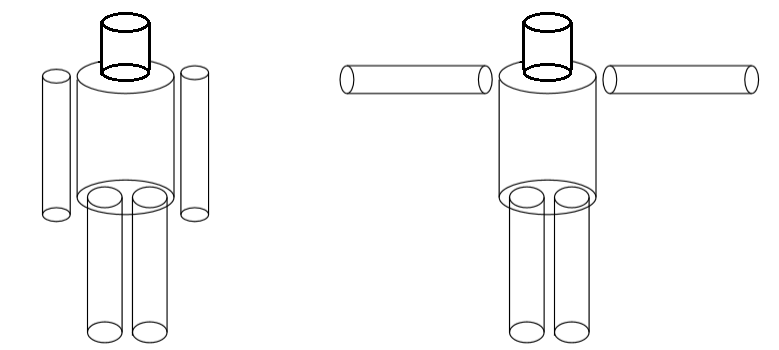
\includegraphics[width=0.3\textwidth]{puppe.PNG}
 \caption{Darstellung der Puppe mit Zylindern \cite{skript} }
 \label{fig:puppe}
 \end{figure}
Die gemessenen Werte werden gemittelt und es ergeben sich folgende Werte für die einzelnen Zylinder:
\begin{table}
  \centering
  \caption{Gemittelter Durchmesser und gemittelte Länge der einzelnen Zylinder}
  \label{tab:puppegemittelt}
  \begin{tabular}{c c c}
    \toprule
    $ $ & Höhe$/\si{\meter}$ & $Durchmesser / \si{\meter}$\\
    \midrule
    Beine & 0.2327\pm 0.0003 & 0.021\pm0.004 \\
    Arme  & 0.181\pm 0.002 & 0.016\pm 0.003 \\
    Kopf  & 0.0772\pm 0.0.0005 & 0.03\pm 0.01 \\
    Torso & 0.122\pm 0.001 & 0.045\pm 0.008 \\
    \bottomrule
   \end{tabular}
\end{table}
Mit der Masse der Puppe $m_{ges}= (0,3407\pm0,0005)\si{\kilo\gram}$
und dem gesamt Volumen $V_{ges}=(0,0005\pm0,0001)\si{\meter\tothe{3}}$
ergibt sich mit:
\begin{align}
  \rho=\frac{m}{V}
\end{align}
eine Dichte von $\rho=(7,4\pm1,6)\si{\kilo\gram\meter\tothe{-3}}$\\
\\
Mit diesen Ergebnissen lässt sich das gesamt Trägheitsmoment $I_{ges}$ bestimmen,
dies ergibt sich aus den einzelnen Trägheitsmomenten der Zylinder, diese lassen sich mit Hilfe der Formel \eqref{eqn:zs}
und des Steinerschen Satzes bestimmen. Für das gesamt Trägheitsmoment ergibt sich:
\begin{align}
  I_{ges}=I_{Kopf}+I_{Torso}+2\cdot I_{Arm}+2\cdot I_{Bein}
\end{align}
Der Zahlenwert ist in Tabelle \ref{tab:puppegrade} zusammen mit den, aus den Messwerten, nach Formel \eqref{eqn:I} berechneten
Trägheitsmomenten zu finden.
\begin{table}
  \centering
  \caption{Schwingdauer, gemessenes und theoretisches Trägheitsmoment der Puppe ohne ausgestreckte Arme}
  \label{tab:puppegrade}
  \begin{tabular}{c c c}
    \toprule
$Schwingdauer/\si{\second}$ & $I_{gemessen}/\si{\kilo\gram\meter\tothe{2}}$ & $I_{theorie}/ \si{\meter}$\\
    \midrule
    0,550\pm0,1   &  -0,0024\pm0,0001   &  0,00011\pm0,00003\\
    0,640\pm0,1   &  -0,0023\pm0,0002   &  0,00011\pm0,00003\\
    0,652\pm0,1   &  -0,0023\pm0,0002   &  0,00011\pm0,00003\\
    0,654\pm0,1   &  -0,0023\pm0,0002   &  0,00011\pm0,00003\\
    0,658\pm0,1   &  -0,0023\pm0,0002   &  0,00011\pm0,00003\\
    0,630\pm0,1   &  -0,0023\pm0,0002   &  0,00011\pm0,00003\\
    0,664\pm0,1   &  -0,0023\pm0,0002   &  0,00011\pm0,00003\\
    0,700\pm0,1   &  -0,0022\pm0,0002   &  0,00011\pm0,00003\\
    0,698\pm0,1   &  -0,0022\pm0,0002   &  0,00011\pm0,00003\\
    0,682\pm0,1   &  -0,0022\pm0,0002   &  0,00011\pm0,00003\\
    \bottomrule
   \end{tabular}
\end{table}
Analog wird dies Für den Körper mit ausgestreckten Armen gehandhabt, hierbei verändert sich das Trägheitsmoment der Arme, dieses berechnet sich hier mit Hilfe von Formel \eqref{eqn:zl}.
Der Theoretische und die mit Messwerten errechneten Werte finden sich in Tabelle \ref{tab:puppeausgestreckt}
\begin{table}
  \centering
  \caption{Schwingdauer, gemessenes und theoretisches Trägheitsmoment der Puppe mit ausgestreckten Armen}
  \label{tab:puppeausgestreckt}
  \begin{tabular}{c c c}
    \toprule
$Schwingdauer/\si{\second}$ & $I_{gemessen}/\si{\kilo\gram\meter\tothe{2}}$ & $I_{theorie}/ \si{\meter}$\\
    \midrule
    1.11\pm0.1  &  -0.0014\pm0.0004  &  0.0007\pm0.0002\\
    1.09\pm0.1  &  -0.0014\pm0.0004  &  0.0007\pm0.0002\\
    1.08\pm0.1  &  -0.0014\pm0.0004  &  0.0007\pm0.0002\\
    1.12\pm0.1  &  -0.0014\pm0.0004  &  0.0007\pm0.0002\\
    1.11\pm0.1  &  -0.0014\pm0.0004  &  0.0007\pm0.0002\\
    1.12\pm0.1  &  -0.0014\pm0.0004  &  0.0007\pm0.0002\\
    1.12\pm0.1  &  -0.0013\pm0.0004  &  0.0007\pm0.0002\\
    1.09\pm0.1  &  -0.0014\pm0.0004  &  0.0007\pm0.0002\\
    1.10\pm0.1  &  -0.0014\pm0.0004  &  0.0007\pm0.0002\\
    1.08\pm0.1  &  -0.0014\pm0.0004  &  0.0007\pm0.0002\\
    \bottomrule
   \end{tabular}
\end{table}
